% mainfile: ../../../../master.tex
\subsection{RNA quantification Nanodrop}
% The part of the label after the colon must match the file name. Otherwise,
% conditional compilation based on task labels does NOT work.
\label{task:20180104_cj2}
\tags{lab,rna,qnt}
\authors{cj}
%\files{}
%\persons{}

For the NanoDrop, I used 2\uL of my sample.

\begin{table}[H]
\caption{../mime/res/nanodrop/CJ20180104.txt}
\label{tab:CJ20180104}
\centering
\begin{tabular}{l l l l l l l l l l l l l }
\toprule
Sample ID & Time  & ng/ul  & A260  & A280  & 260/280  & 260/230  \\ \midrule
\texttt{CJ20180103\_BLANK} & 17:25 & 0,20 & 0,004 & 0,010 & 0,41 & 0,56 \\
\texttt{CJ20180103\_RNA} & 17:26 & 52,5 & 1,313 & 0,893 & 1,47 & 0,28 \\
\texttt{CJ20180103\_DNA} & 17:28 & 52,9 & 1,057 & 0,674 & 1,57 & 0,19 \\

\bottomrule
\end{tabular}
\\
User: Default - Date: 04.01.2018 - Constant: 50,00 - Cursor position: 230 \
\end{table}

% Figures
\begin{figure}[H] % position of the figure 
    \centering
    \caption{Screenshots of the NanoDrop analysis of RNA samples extracted from liquid culture}
    \label{fig:label}
    \begin{subfigure}[b]{0.49\textwidth}
        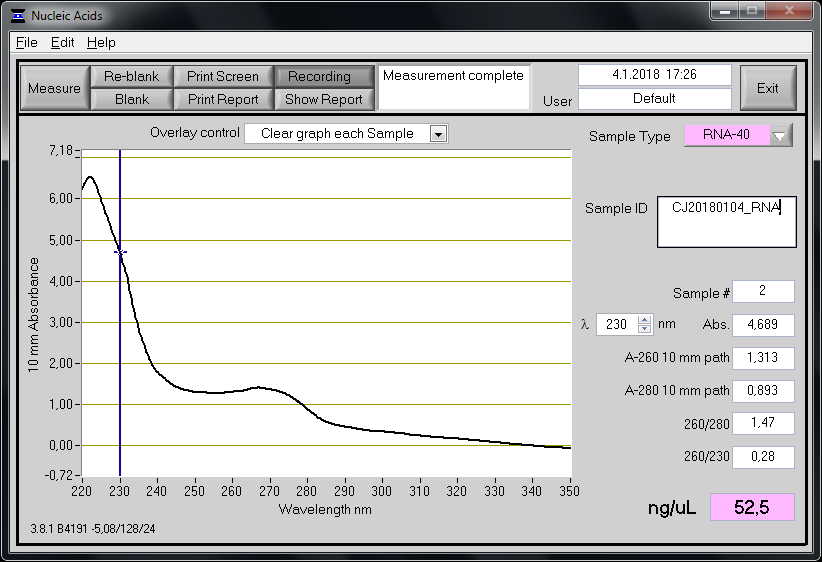
\includegraphics[width=\textwidth]{graphics/screenshots/CJ20180104_RNA.png}
        \caption{Calculating RNA concentration.}
        \label{sfig:CJ20180104_RNA}
    \end{subfigure}
    ~ 
    \begin{subfigure}[b]{0.49\textwidth}
        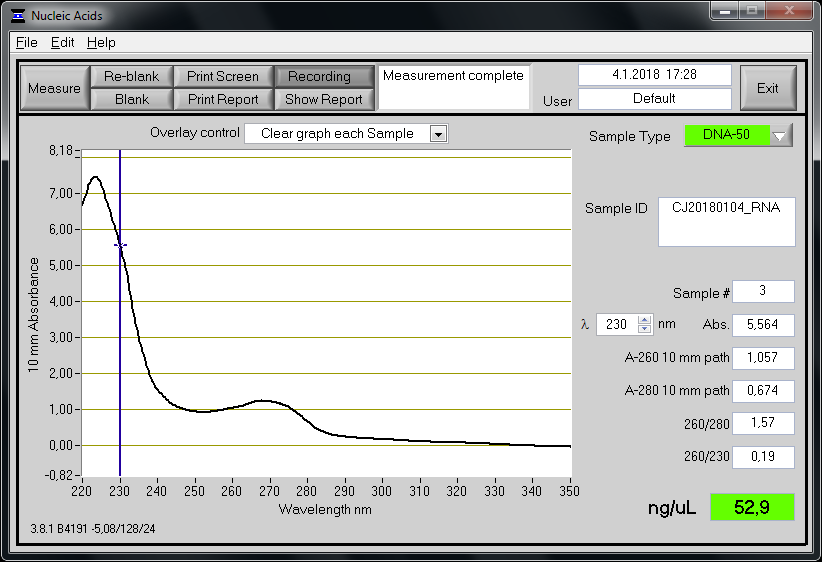
\includegraphics[width=\textwidth]{graphics/screenshots/CJ20180104_RNA_asDNA.png}
        \caption{Calculating DNA concentration.}
        \label{sfig:CJ20180104_RNA_asDNA}
    \end{subfigure}
\end{figure}
